%!TEX root = mainfile.tex

\section{Cosmic Variance} % (fold)
\label{sec:cosmic_variance}
(Lewis with contributions from Andrew)

	In general, the Universe can only be considered to be homogeneous at the most extreme distance scales ($>\SI{1}{\giga\parsec}$). At the scales which tend to be observed, matter in the Universe is not distributed uniformly and will gather together in massive clusters. Conversely, there will be empty regions of space known as voids where virtually no matter is present at all.

	Measurements deduced from observational surveys will certainly be affected by this large-scale cosmic structure. A measurement of an arbitrary region of the sky will have an associated uncertainty far greater than any sample variance due to Poisson statistics. This uncertainty is known as \emph{Cosmic Variance}, and will nearly always be the dominant source of error for any high-redshift cosmic survey. Given a probability distribution for the number counts, the cosmic variance is defined as
	\begin{align}
		\sigma_v^2= \frac{\left \langle N^2 \right \rangle - \left \langle N \right \rangle^2}{\left \langle N \right \rangle}-\frac{1}{\left \langle N \right \rangle} \label{eq:cvstat}
	\end{align}
	where $\left \langle N \right \rangle$ is the mean and $\left \langle N^2 \right \rangle$ is the variance\cite{Trenti2008}.

	Any number or density measurement derived from a galaxy population is susceptible to cosmic variance. As an extreme example, it is reported to be potentially at the 50--70\% level in the HST UDF surveys\cite{Driver01102010}. Evidently, it will be particularly relevant to this study of cosmic reionization.

	\subsection{Factors which affect the Cosmic Variance} % (fold)
	\label{sub:factors_which_affect_the_cosmic_variance}
		Fortunately, there exist numerous ways of reducing the cosmic variance of a galaxy survey to a manageable amount, mostly accepted to be $<10\%$. As a general rule, this is achieved when a volume of \SI{e7}{\mega\parsec\cubed} is surveyed, with a square survey area over a single contiguous region\cite{Driver01102010}.

		The cosmic variance of a survey principally depends on three factors. It will
		\begin{itemize}
			\item decrease steadily as the survey volume gets larger,
			\item be reduced for higher aspect ratio surveys,
			\item be reduced when multiple sight-lines are taken i.e.\ sparse sampling.
		\end{itemize}
		Taking advantage of these factors, one can take steps to address the issue of cosmic variance.
	% subsection factors_which_affect_the_cosmic_variance (end)

		\subsubsection{Survey Volume} % (fold)
		\label{ssub:survey_volume}
			As mentioned above, the cosmic variance is heavily dependent on the volume of the survey, indicated by the steady decrease to lower percentages as larger volumes are surveyed, as in Figure~\ref{fig:cv1}. It can be seen that for volumes of \SI{e4}{\mega\parsec\cubed}, it is as much as 60\% whereas for \SI{e7}{\mega\parsec\cubed}, it will be 10\% and below.

			The dashed line below the main trend on the graph in Figure~\ref{fig:cv1} shows how the percentage uncertainty varies solely due to the sample variance. This gives some idea of the gulf between the effect of cosmic variance and that of Poisson statistics.
			\begin{figure}
				\centering
				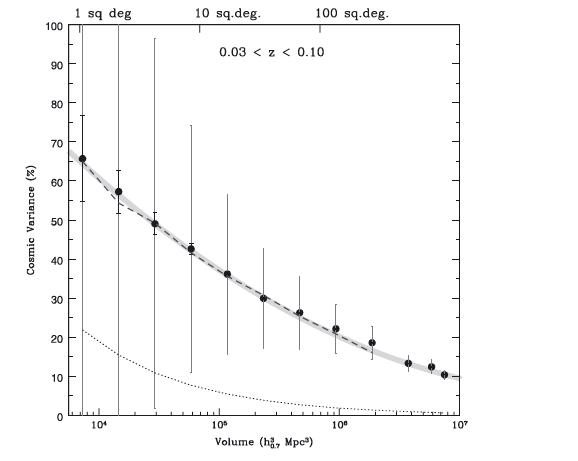
\includegraphics[width=0.7\textwidth]{../Images/cosmic_variance1.JPG}
				\caption{Graph showing the relation between the percentage cosmic variance and survey volume.\label{fig:cv1}}
			\end{figure}

			\begin{figure}
				\centering
				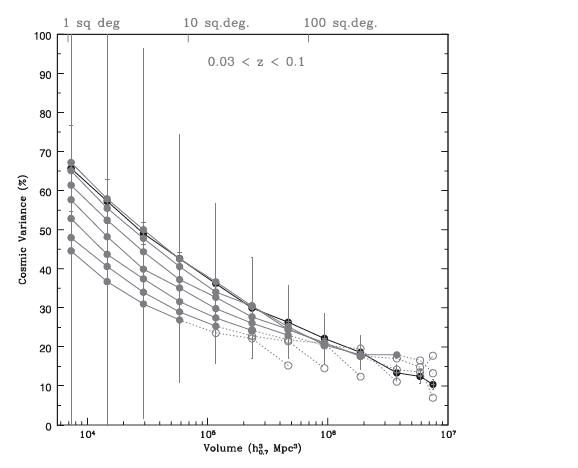
\includegraphics[width=0.7\textwidth]{../Images/cosmic_variance2.JPG}
				\caption{The same as for graph 1, this time with the additional grey points showing the dependence on aspect ratio. From the top to bottom they are 1:2, 1:4, 1:8, 1:16, 1:32, 1:64 and 1:128.}\label{fig:cv2}
			\end{figure}
		% subsubsection survey_volume (end)

		\subsubsection{Aspect Ratio} % (fold)
		\label{ssub:aspect_ratio}
			The aspect ratio of the survey is another crucial factor that can help deal with cosmic variance. For the same survey area, a long thin strip chosen over a standard square-shaped survey will decrease the cosmic variance. When taken to the extreme, this can cause a significant reduction. The same trend as for Figure~\ref{fig:cv1} is shown in Figure~\ref{fig:cv2}, but with the grey dots corresponding to higher aspect ratio surveys. The graph illustrates that, particularly for larger volumes, increasing the aspect ratio of a survey can make a huge reduction in the cosmic variance uncertainty.
		% subsubsection aspect_ratio (end)

		\subsubsection{Sparse Sampling} % (fold)
		\label{ssub:sparse_sampling}
			One might tackle cosmic variance in a very effective manner via the method of \emph{sparse sampling} whereby several identical observing areas are distributed randomly across the sky. As opposed to one contiguous survey, these multiple sight-lines in different directions allow a more representative portion of the sky to be surveyed.

			It has been shown that cosmic variance is reduced with the number, $N$ of such sight-lines by $\frac{1}{\sqrt{N}}$. This holds irrespective of the base survey area\cite{Driver01102010}.
		% subsubsection sparse_sampling (end)

	\subsection{General Formula} % (fold)
	\label{sub:general_formula}
		In order to address cosmic variance in the code itself, an empirical formula was employed. In a paper (Driver and Robotham, 2010), this formula was derived using data from the Sloan Digital Sky Survey (SDSS), and extrapolated out to higher redshifts\cite{Driver01102010}. Due to its extrapolated nature, it should be noted that this is an approximate formula. Nonetheless, it should output a robust estimate of the cosmic variance for given surveys. Additionally, through it one can deduce possible ways to reduce the cosmic variance to below 10\%.
		\begin{align}
			\zeta _{CV}(\%)=\frac{\left( 1.00-0.03\sqrt{X-1} \right)\times \left( 219.7-52.4\log_{10}\left(291.0\times AB \right) + 3.21\log_{10}{\left(291.0\times AB\right)}^{2} \right)}{\sqrt{NC/291.0}} \label{eq:cvmain}
		\end{align}
		The formula employs the median redshift transverse lengths $A$ and $B$, and the radial depth $C$, all given in \si{\mega\parsec}, to represent the volume of each survey sample. The number of such samples i.e.\ the number of sight-lines is $N$. The aspect ratio is dealt with in the amplitude term at the front of the expression, where the aspect ratio 1:128 would be submitted as $X=128$, for example.

		Although it is extrapolated from an equation that applies at $z<0.1$, it takes advantage of the fact that cosmic variance should vary according to Poisson statistics along the radial length. This means that a survey with twice the radial depth will have $\sqrt{2}$ less cosmic variance. Hence the factor of $\sqrt{C}$ in the denominator. equation~(\ref{eq:cvmain}) does not, however, make any corrections for the evolution of the clustering signature of the galaxy population, with this expected to be lower towards higher redshift. Correspondingly, any estimate output should be treated as an upper limit.

		This equation has been entered into the code which, from the survey parameters input, calculates the required quantities and gives an estimate of the cosmic variance as a percentage of the number counts expected to be observed. Furthermore, it will inform the user of how many random pointings of such a survey are necessary to achieve less than $10\%$ cosmic variance.
	% subsection general_formula (end)
% section cosmic_variance (end)

%written and researched by Lewis Clegg, coded by Andy King.
